\pdfminorversion=4
\documentclass[aspectratio=169]{beamer}

\mode<presentation>
{
  \usetheme{default}
  \usecolortheme{default}
  \usefonttheme{default}
  \setbeamertemplate{navigation symbols}{}
  \setbeamertemplate{caption}[numbered]
  \setbeamertemplate{footline}[frame number]  % or "page number"
  \setbeamercolor{frametitle}{fg=white}
  \setbeamercolor{footline}{fg=black}
}

\usepackage[english]{babel}
\usepackage[utf8x]{inputenc}
\usepackage{tikz}
\usepackage{courier}
\usepackage{array}
\usepackage{bold-extra}
\usepackage{minted}
\usepackage[thicklines]{cancel}
\usepackage{fancyvrb}

\xdefinecolor{dianablue}{rgb}{0.18,0.24,0.31}
\xdefinecolor{darkblue}{rgb}{0.1,0.1,0.7}
\xdefinecolor{darkgreen}{rgb}{0,0.5,0}
\xdefinecolor{darkgrey}{rgb}{0.35,0.35,0.35}
\xdefinecolor{darkorange}{rgb}{0.8,0.5,0}
\xdefinecolor{darkred}{rgb}{0.7,0,0}
\definecolor{darkgreen}{rgb}{0,0.6,0}
\definecolor{mauve}{rgb}{0.58,0,0.82}

\title[2019-05-15-refinement-types-irishep]{Refinement types and other werid language features for physics}
\author{Jim Pivarski}
\institute{Princeton University -- IRIS-HEP}
\date{May 15, 2019}

\usetikzlibrary{shapes.callouts}

\begin{document}

\logo{\pgfputat{\pgfxy(0.11, 7.4)}{\pgfbox[right,base]{\tikz{\filldraw[fill=dianablue, draw=none] (0 cm, 0 cm) rectangle (50 cm, 1 cm);}\mbox{\hspace{-8 cm}
\includegraphics[height=1 cm]{princeton-logo-long.png}\hspace{0.1 cm}\raisebox{0.1 cm}{
\includegraphics[height=0.8 cm]{iris-hep-logo-long.png}}\hspace{0.1 cm}}}}}

\begin{frame}
  \titlepage
\end{frame}

\logo{\pgfputat{\pgfxy(0.11, 7.4)}{\pgfbox[right,base]{\tikz{\filldraw[fill=dianablue, draw=none] (0 cm, 0 cm) rectangle (50 cm, 1 cm);}\mbox{\hspace{-8 cm}
\includegraphics[height=1 cm]{princeton-logo.png}\hspace{0.1 cm}\raisebox{0.1 cm}{
\includegraphics[height=0.8 cm]{iris-hep-logo.png}}\hspace{0.1 cm}}}}}

% Uncomment these lines for an automatically generated outline.
%\begin{frame}{Outline}
%  \tableofcontents
%\end{frame}

% START START START START START START START START START START START START START

\begin{frame}{}
\large
\vspace{1.25 cm}
Quite a few groups have been thinking about physics event processing languages, explicitly or implicitly.

\vspace{0.25 cm}
\begin{itemize}
\item \textcolor{darkblue}{LHADA/ADL:} Sezen Sekmen, Harry Prosper, Philippe Gras
\item \textcolor{darkblue}{CutLang:} Gokhan Unel
\item \textcolor{darkblue}{IRIS-HEP Analysis Systems:} Gordon Watts, Mason Proffitt, Emma Torro
\item \textcolor{darkblue}{FAST-Carpenter (YAML):} Benjamin Krikler
\item \textcolor{darkblue}{NAIL:} Andrea Rizzi
\item \textcolor{darkblue}{RDataFrame:} Enrico Guiraud, Danilo Piparo, and the ROOT Team
\item \textcolor{darkblue}{AEACuS \& RHADAManTHUS:} Joel Walker (phenomenology)
\item \textcolor{darkblue}{Femtocode:} me, though not for several years\ldots
\end{itemize}

\vspace{0.25 cm}
\small \hfill see \textcolor{blue}{\href{https://indico.cern.ch/event/769263/timetable/}{Analysis Description Languages Workshop}} (May 6--8)
\end{frame}

\begin{frame}{}
\Large
\vspace{1.25 cm}
\begin{center}
Originally, I was going to talk about refinement types \\ (a core feature of Femtocode), but this talk has grown.
\end{center}
\end{frame}

\begin{frame}{}
\vspace{1.25 cm}
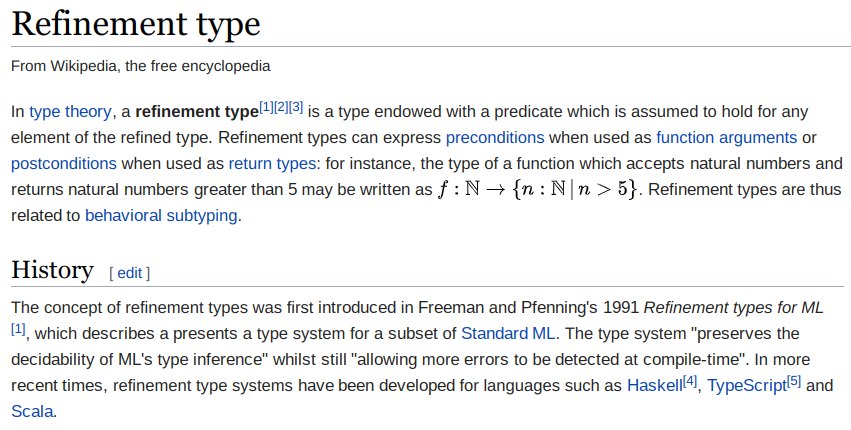
\includegraphics[width=\linewidth]{refinement-wikipedia.png}
\end{frame}

\begin{frame}[fragile]{Example in practice: \only<1-2>{prevent NaN at compile-time}\only<3-4>{identify impossible situations}}
\begin{columns}
\column{1.1\linewidth}
\begin{center}
\only<1>{\fbox{\mintinline{python}{x / y}}}\only<2>{\fbox{\mintinline{python}{if y != 0: x / y else: None}}}\only<3>{\fbox{\mintinline{python}{x == 5 and y == 6 and x == y}}}\only<4>{\fbox{\mintinline{python}{x == y and x == 5 and y == 6}}}
\end{center}

\begin{onlyenv}<1>
\begin{verbatim}
femtocode.parser.FemtocodeError: Function "/" does not accept
arguments with the given types:

    /(real,
      real)

    Indeterminate form (0 / 0) is possible; constrain with if-else.

Check line:col 1:0 (pos 0):

    x / y
----^
\end{verbatim}
\end{onlyenv}
\begin{onlyenv}<2>
\begin{verbatim}
----> union(null, real)











\end{verbatim}
\end{onlyenv}
\begin{onlyenv}<3>
\begin{verbatim}
femtocode.parser.FemtocodeError: Function "==" does not accept
arguments with the given types:

    ==(integer(min=5, max=5),
       integer(min=6, max=6))

    The argument types have no overlap (values can never be equal).

Check line:col 1:27 (pos 27):

    x == 5 and y == 6 and x == y
-------------------------------^
\end{verbatim}
\end{onlyenv}
\begin{onlyenv}<4>
\begin{verbatim}
femtocode.parser.FemtocodeError: Function "==" does not accept
arguments with the given types:

    ==(integer(min=5, max=5),
       integer(min=6, max=6))

    The argument types have no overlap (values can never be equal).

Check line:col 1:5 (pos 5):

    x == y and x == 5 and y == 6
---------^
\end{verbatim}
\end{onlyenv}
\end{columns}
\end{frame}

\begin{frame}{It's possible to turn {\it all} runtime errors into compile errors}
\large
\vspace{0.4 cm}
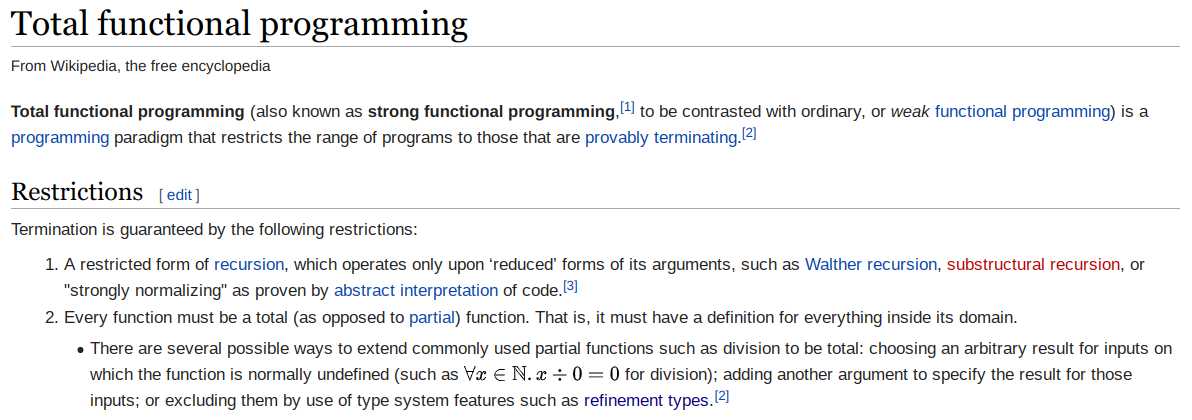
\includegraphics[width=0.98\linewidth]{totalfunctional-wikipedia.png}

\vspace{0.25 cm}
Including value sets in the type definitions lets us identify runtime conditions in the type-check.

\vspace{0.25 cm}
The hard parts are recursion (structural recursion) and infinite datasets (codata), both of which we can safely exclude from physics event processing.
\end{frame}

\begin{frame}[fragile]{Even without {\it total} functions, it can be useful for array lengths}
\large
\vspace{0.5 cm}

Awkward-Array users sometimes make this mistake:

\small\begin{minted}{python}
(nMuons > 0) & (Muons_pt[:, 0] > 30)    # intersection of masks
\end{minted}
\large

\vspace{0.25 cm}
The first mask requires events with at least one muon and the second requires the first muon to have 30~GeV, {\it but the selections are independent,} so the second fails at runtime when some events have no muons.

\vspace{0.5 cm}
\begin{uncoverenv}<2->
The right way to do it is with a single selection:

\small\begin{minted}{python}
Muons_pt[(nMuons > 0), 0] > 30          # mask first dim, pick 0
\end{minted}
\end{uncoverenv}

\large

\vspace{0.25 cm}
\uncover<3->{\textcolor{darkblue}{This error would be safer and more informative as a type error.}}
\end{frame}

\begin{frame}{Minimal application of refinement types}
\Large
\vspace{0.25 cm}
\begin{center}
It would be useful for an array's type description to include bounds on its length---minimally, whether it could be empty or not.

\large
\vspace{0.5 cm}
\begin{minipage}{0.85\linewidth}
\begin{itemize}
\item Some languages (e.g.\ Numba) already include an array's dimension in its type.
\item Some functions, like integer {\tt min}/{\tt max} or {\tt argmin}/{\tt argmax}, don't have a good runtime solution for empty arrays.
\item Some arrays, such as those coming from a group-by operations, can be guaranteed non-empty.
\item Functional operations, like {\tt map}, {\tt filter}, and {\tt joins}, transform array lengths in semi-predictable ways.
\end{itemize}
\end{minipage}
\end{center}
\end{frame}

\begin{frame}[fragile]{Other weird language features}
\Large
\vspace{0.5 cm}

\underline{Pattern matching}: like regular expressions for data structures.

\vspace{0.65 cm}
\textcolor{darkorange}{\bf Scala:}

\begin{center}
\begin{minipage}{0.85\linewidth}
\normalsize
\begin{minted}{scala}
def pz(particle: Particle) = match particle {
    case Neutral(pt, eta, _)    => pt * sinh(eta)
    case Charged(pt, eta, _, q) => pt * sinh(eta)
}
\end{minted}
\end{minipage}
\end{center}

\vspace{0.25 cm}
\textcolor{darkorange}{\bf Haskell:}

\begin{center}
\begin{minipage}{0.85\linewidth}
\normalsize
\begin{minted}{haskell}
pz :: (Particle particle) => particle -> Float
pz (Neutral pt eta _)   = pt * sinh(eta)
pz (Charged pt eta _ q) = pt * sinh(eta)
\end{minted}
\end{minipage}
\end{center}
\end{frame}

\begin{frame}{Pattern matching}
\LARGE
\vspace{0.5 cm}
\begin{center}
Could we use pattern matching to associate \\ particle candidates to a given decay chain?
\end{center}
\end{frame}

\begin{frame}[fragile]{Something like this?}
\begin{Verbatim}[commandchars=\\\{\}]
Higgs \{
    Z1 \{
        lep1, lep2 \textcolor{blue}{in} \textcolor{darkgreen}{electrons} \textcolor{blue}{or} lep1, lep2 \textcolor{blue}{in} \textcolor{darkgreen}{muons}
        \textcolor{blue}{requiring} lep1.\textcolor{mauve}{charge} != lep2.\textcolor{mauve}{charge}
    \}
    Z2 \{
        lep3, lep4 \textcolor{blue}{in} \textcolor{darkgreen}{electrons} \textcolor{blue}{or} lep3, lep4 \textcolor{blue}{in} \textcolor{darkgreen}{muons}
        \textcolor{blue}{requiring} lep3.\textcolor{mauve}{charge} != lep4.\textcolor{mauve}{charge}
    \}
    \textcolor{blue}{minimizing} (Z1.\textcolor{mauve}{mass} - \textcolor{darkorange}{91})**2 + (Z2.\textcolor{mauve}{mass} - \textcolor{darkorange}{91})**2
\}
\end{Verbatim}

\large
\vspace{0.5 cm}
where the match ensures that leptons aren't double-counted in both Z's?
\end{frame}

\begin{frame}[fragile]{Or, what about this?}
\Large
\vspace{0.5 cm}
Behold Racket (Scheme)'s two-dimensional syntax!

\normalsize

\vspace{0.25 cm}
\begin{center}
\begin{minipage}{0.8\linewidth}
\begin{minted}{scheme}
(define (subtype? a b)
  #2dmatch
  +----------+----------+-------+----------+
  |   a  b   | 'Integer | 'Real | 'Complex |
  +----------+----------+-------+----------+
  | 'Integer |             #t              |
  +----------+----------+                  |
  | 'Real    |          |                  |
  +----------+          +-------+          |
  | 'Complex |        #f        |          |
  +----------+------------------+----------+)
\end{minted}
\end{minipage}
\end{center}

\vspace{0.25 cm}
\small \hfill see \textcolor{blue}{\href{https://docs.racket-lang.org/2d/index.html}{Racket documentation}}
\end{frame}

\begin{frame}[fragile]{So maybe something like this?}
\begin{Verbatim}[commandchars=\\\{\}]
Higgs : \textcolor{blue}{fit} (Z1.\textcolor{mauve}{mass} - \textcolor{darkorange}{91})**2 + (Z2.\textcolor{mauve}{mass} - \textcolor{darkorange}{91})**2
   |
   +--> Z1 : \textcolor{blue}{cut} lep1.\textcolor{mauve}{charge} != lep2.\textcolor{mauve}{charge}
   |     |
   |     +--> lep1, lep2 \textcolor{blue}{in} \textcolor{darkgreen}{electrons} \textcolor{blue}{or} lep1, lep2 \textcolor{blue}{in} \textcolor{darkgreen}{muons}
   |
   +--> Z2 : \textcolor{blue}{cut} lep3.\textcolor{mauve}{charge} != lep4.\textcolor{mauve}{charge}
         |
         +--> lep3, lep4 \textcolor{blue}{in} \textcolor{darkgreen}{electrons} \textcolor{blue}{or} lep3, lep4 \textcolor{blue}{in} \textcolor{darkgreen}{muons}
\end{Verbatim}

\large
\vspace{0.5 cm}
Maybe the arrows are unnecessary; maybe an indentation rule like Python's\ldots
\end{frame}

\begin{frame}[fragile]{I tried out some ideas with a simple parser and interpreter}
\Large
\vspace{0.5 cm}
\textcolor{blue}{\small \url{https://github.com/diana-hep/rejig/blob/master/pattern-match/define-and-run.py}}

\vspace{0.5 cm}
\only<1>{\textcolor{darkblue}{Syntax:}}\only<2>{\textcolor{darkblue}{Example:}}

\begin{center}
\begin{minipage}{0.85\linewidth}
\normalsize
\begin{onlyenv}<1>
\begin{Verbatim}[commandchars=\\\{\}]
\textcolor{darkgreen}{pattern:}    derivation* constraint* \textcolor{darkorange}{"for"} multiple
\textcolor{darkgreen}{derivation:} CNAME \textcolor{darkorange}{"="} expression
\textcolor{darkgreen}{constraint:} \textcolor{darkorange}{"if"} expression -> if
          | \textcolor{darkorange}{"best"} expression -> best
          | \textcolor{darkorange}{"sort"} expression -> sort
\textcolor{darkgreen}{multiple:}   single (\textcolor{darkorange}{","} single)*
\textcolor{darkgreen}{single:}     CNAME (\textcolor{darkorange}{","} CNAME)* \textcolor{darkorange}{"in"} expression
\end{Verbatim}
\vspace{\baselineskip}
\end{onlyenv}
\begin{onlyenv}<2>
\vspace{-0.5\baselineskip}
\begin{Verbatim}[commandchars=\\\{\}]
higgs2e2mu = \textcolor{blue}{match} \{
    z1 = lep1 + lep2
    z2 = lep3 + lep4
    hmass = \textcolor{mauve}{mass}(z1 + z2)
    \textcolor{blue}{if} lep1.\textcolor{mauve}{charge} != lep2.\textcolor{mauve}{charge}
    \textcolor{blue}{if} lep3.\textcolor{mauve}{charge} != lep4.\textcolor{mauve}{charge}
    \textcolor{blue}{for} lep1, lep2 \textcolor{blue}{in} electrons, lep3, lep4 \textcolor{blue}{in} muons
\}
\end{Verbatim}
\end{onlyenv}
\end{minipage}
\end{center}

\normalsize \uncover<1>{and normal expression syntax (math operations, comparisons, etc.).}
\end{frame}

\begin{frame}[fragile]{Complete example: same flavor and opposite flavor dileptons}
\scriptsize
\vspace{0.25 cm}
\begin{Verbatim}[commandchars=\\\{\}]
\textcolor{mauve}{mass}(particle) = \textcolor{mauve}{sqrt}(particle.\textcolor{mauve}{E}**\textcolor{darkorange}{2} - particle.\textcolor{mauve}{px}**\textcolor{darkorange}{2} - particle.\textcolor{mauve}{py}**\textcolor{darkorange}{2} - particle.\textcolor{mauve}{pz}**\textcolor{darkorange}{2})

\textcolor{mauve}{same_flavor}(collection) = \textcolor{blue}{match} \{
    z1 = lep1 + lep2; z2 = lep3 + lep4
    hmass = \textcolor{mauve}{mass}(z1 + z2)
    \textcolor{blue}{if} lep1.\textcolor{mauve}{charge} != lep2.\textcolor{mauve}{charge}
    \textcolor{blue}{if} lep3.\textcolor{mauve}{charge} != lep4.\textcolor{mauve}{charge}
    \textcolor{blue}{sort} (\textcolor{mauve}{mass}(z1) - \textcolor{darkorange}{91})**\textcolor{darkorange}{2} + (\textcolor{mauve}{mass}(z2) - \textcolor{darkorange}{91})**\textcolor{darkorange}{2}
    \textcolor{blue}{for} lep1, lep2, lep3, lep4 \textcolor{blue}{in} collection
\}[:\textcolor{darkorange}{1}]   \textcolor{gray}{# at most one}

higgs4e  = \textcolor{mauve}{same_flavor}(electrons)
higgs4mu = \textcolor{mauve}{same_flavor}(muons)

higgs2e2mu = \textcolor{blue}{match} \{
    z1 = lep1 + lep2; z2 = lep3 + lep4                   \textcolor{gray}{# hmmm... repetitive}
    hmass = \textcolor{mauve}{mass}(z1 + z2)
    \textcolor{blue}{if} lep1.\textcolor{mauve}{charge} != lep2.\textcolor{mauve}{charge}
    \textcolor{blue}{if} lep3.\textcolor{mauve}{charge} != lep4.\textcolor{mauve}{charge}
    \textcolor{blue}{sort} (\textcolor{mauve}{mass}(z1) - \textcolor{darkorange}{91})**\textcolor{darkorange}{2} + (\textcolor{mauve}{mass}(z2) - \textcolor{darkorange}{91})**\textcolor{darkorange}{2}
    \textcolor{blue}{for} lep1, lep2 \textcolor{blue}{in} electrons, lep3, lep4 \textcolor{blue}{in} muons     \textcolor{gray}{# only line that's different}
\}[:\textcolor{darkorange}{1}]   \textcolor{gray}{# at most one}
\end{Verbatim}
\end{frame}

\begin{frame}[fragile]{A good language construct can be used for other purposes}
\Large
\vspace{0.25 cm}

How about matching generator-level and reconstructed particles?

\vspace{0.25 cm}
{\normalsize (Or matching jets from different algorithms, or computing isolation variables, etc.)}

\normalsize
\vspace{0.25 cm}
\begin{Verbatim}[commandchars=\\\{\}]
genreco = match \{
    if delta_R(gen, reco) < 0.5
    for gen in generator, reco in reconstructed
\}
\end{Verbatim}

\Large
\vspace{0.25 cm}
\begin{uncoverenv}<2->
It's a start, but now we need to group by either {\tt gen} or {\tt reco} and find the best (minimum {\tt delta\_R}) in each group.

\vspace{0.5 cm}
Should grouping be part of the {\tt match} syntax or separate?
\end{uncoverenv}
\end{frame}

\begin{frame}{(Self) Criticisms}
\Large
\vspace{0.5 cm}
\begin{itemize}\setlength{\itemsep}{0.25 cm}
\item This is not so much a pattern-matching syntax as a declarative looping construct.
\item It's starting to look wordy, like SQL (or COBOL).
\item Like SQL and COBOL, it's using special syntax where a chain of functionals would work as well.
\end{itemize}
\end{frame}

\end{document}
